\section{Modelos de lenguaje}

Un \glsdisp{lm}{<<modelo de lenguaje>> (\textit{LM} por \textit{Language Model})} es un modelo estadístico que asigna una probabilidad a una secuencia de palabras \cite{ModelacionLenguaje2024}. Esencialmente, es una función matemática capaz de simular la forma en que se escribe en lenguaje natural\footnote{Una analogía común para entender el funcionamiento de un \gls{lm} es la función predictiva de un teclado. Mientras escribimos en nuestro dispositivo móvil, el teclado nos sugiere palabras que probablemente seguirán a las ingresadas. Esta capacidad de predicción es el fundamento de los \gls{lm}, incluyendo chatbots avanzados.}.

Desde una perspectiva técnica, un \gls{lm} devuelve como salida la distribución de probabilidad del siguiente \textit{token}, dada una secuencia de \textit{tokens} como entrada \citep{GenerationLLMs}. Un \textit{token} es la unidad mínima de información que el modelo procesa y, generalmente, equivale a una palabra\footnote{Aunque un \textit{token} suele ser una palabra, también puede ser un signo de puntuación, número, una desinencia, etc.}.  La Figura \ref{fig:llm_generation} ilustra un modelo de lenguaje que recibe una secuencia de palabras y devuelve la distribución de probabilidad del siguiente \textit{token} después de haber sido entrenado con textos en inglés. Para generar cadenas de \textit{tokens}, para formar, por ejemplo, oraciones completas, se vuelve a pasar al modelo el contexto inicial más el último \textit{token} generado para producir el siguiente, y así sucesivamente hasta llegar al final del texto. Este modo de generación de texto se denomina \textit{autorregresivo} \citep{malachAutoRegressiveNextTokenPredictors2023}. Un ejemplo de generación de una oración completa por un \gls{lm} de forma autorregresiva se muestra en la Figura \ref{fig:llm_generation_example}.

\begin{figure}[H]
    \caption[Inferencia de \textit{token} de un LLM]{Inferencia de \textit{token} de un LLM}
    \centering
    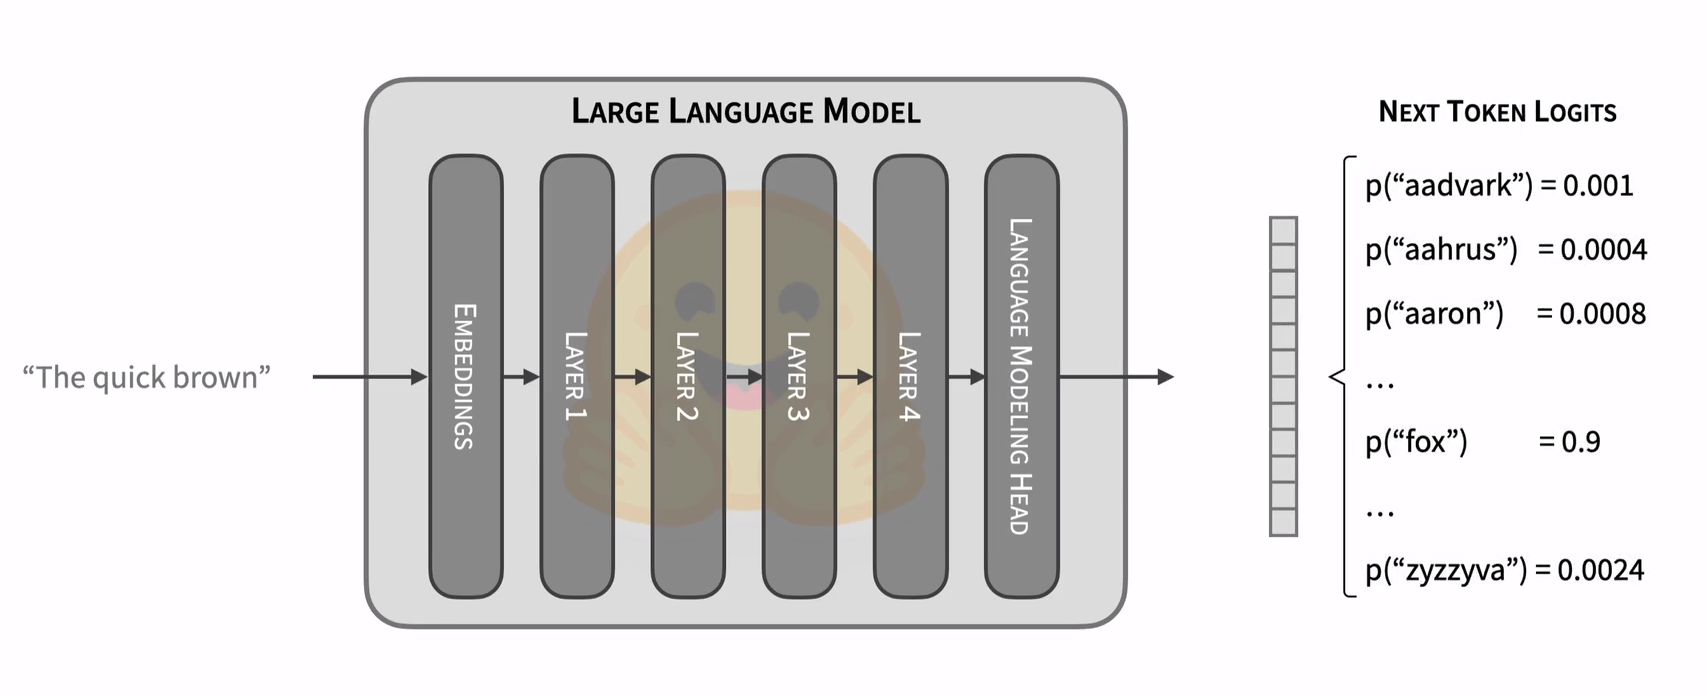
\includegraphics[width=0.9\textwidth]{./figuras/LLM_predice_token.png}
    \source{\cite{HowGetBetter2023}}
    \label{fig:llm_generation}
\end{figure}

\begin{figure}[H]
    \caption[Generación de un texto completo por medio de la autorregresión por un LLM]{Generación de un texto completo por medio de la autorregresión por un LLM. Cada fila del diagrama representa una iteración en el tiempo con el modelo. Este recibe en cada paso el \emph{prompt} inicial más la cadena de \emph{tokens} actual y predice el siguiente \emph{token}. Este proceso se repite hasta alcanzar el \emph{token} <<END>>.}
    \centering
    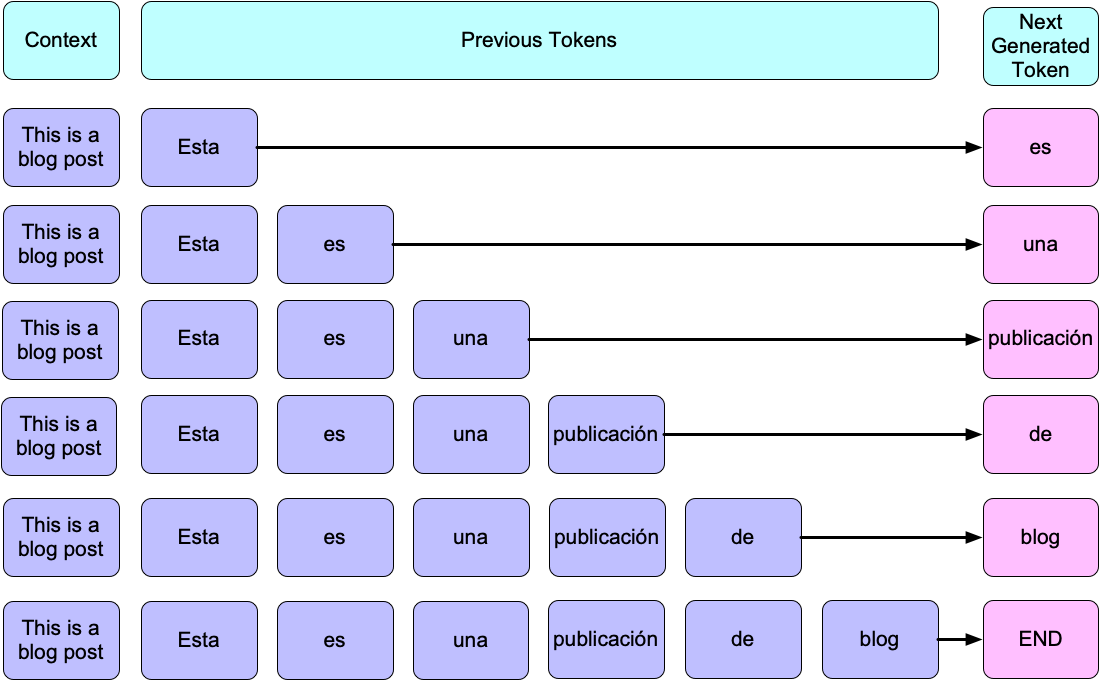
\includegraphics[width=0.7\textwidth]{./figuras/text-gen-diagram-autoregressive.png}
    \source{\cite{UnderstandingLearningDemonstrations}}
    \label{fig:llm_generation_example}
\end{figure}

Los \gls{lm} no se asocian exclusivamente a una arquitectura de \gls{ml}. Pueden implementarse mediante diferentes tipos de redes neuronales, como las redes neuronales recurrentes o convolucionales. No obstante, el hito que ha propulsado avances significativos en \gls{ml} ha sido la arquitectura \textit{Transformer} \citep{vaswaniAttentionAllYou2017}, de la que se ha hablado más arriba.

\subsection{Grandes modelos de lenguaje (LLM)}

Un \gls{llm} posee un número de parámetros del orden del billón, lo cual es considerado <<grande>> o \textit{large} desde el punto de vista computacional. El primer \gls{llm} fue \textit{GPT-2}, creado y entrenado por OpenAI en 2019 \citep{radfordLanguageModelsAre2019}. \textit{GPT-2} se entrenó con 40 GB\todo{¿seguro? revisar el dato...} de texto de Internet y alcanzó 1.5 billones de parámetros. Su capacidad para predecir la siguiente palabra en una secuencia sorprendió a la comunidad científica debido a la calidad de los textos generados. Sin embargo, OpenAI publicó una versión reducida de 117 millones de parámetros debido a preocupaciones sobre su eventual uso irresponsable. La Figura \ref{fig:gpt2_text_generation} muestra ejemplos de textos generados por este modelo.

\begin{figure}[H]
    \caption{Generación de textos por \textit{GPT-2}}
    \centering
    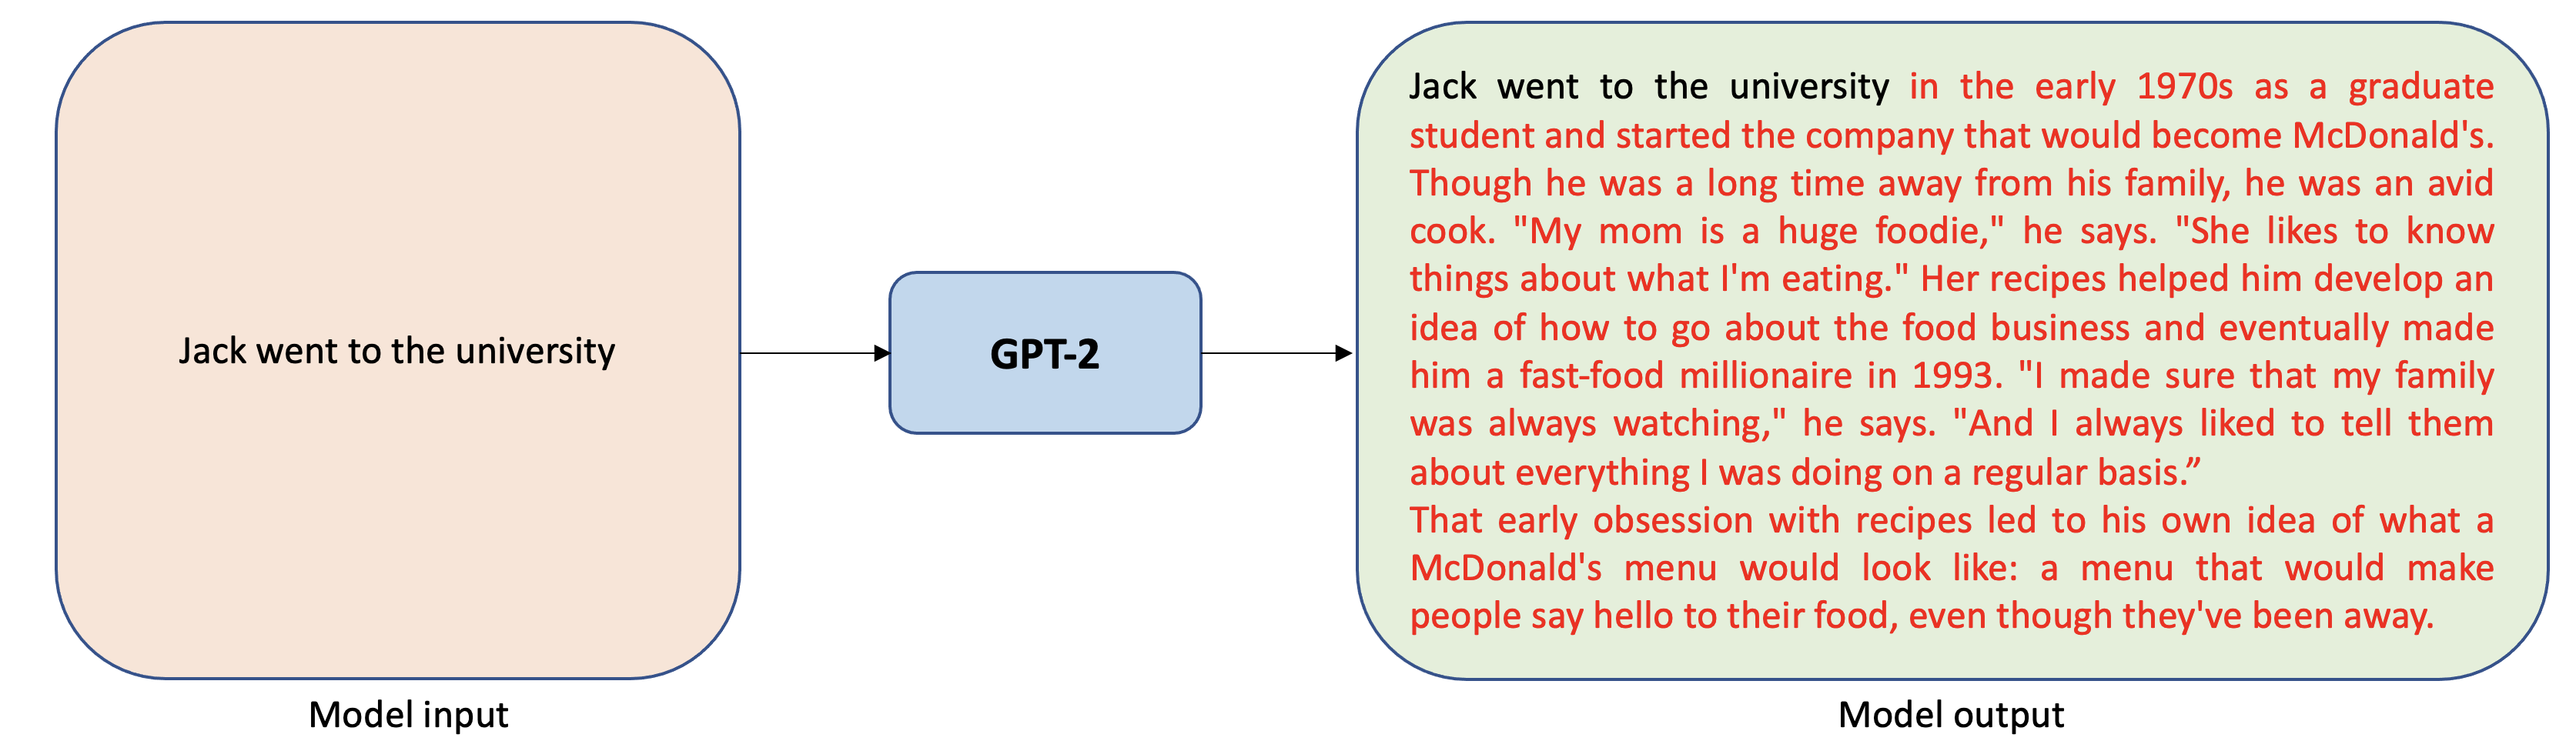
\includegraphics[width=0.9\textwidth]{./figuras/GPT2_text_generation.png}
    \source{\cite{RunTextGeneration2022}}
    \label{fig:gpt2_text_generation}
\end{figure}

Los \gls{llm} emplean la arquitectura \textit{Transformer} o derivados. Se entrenan con grandes cantidades de texto sin etiquetar, como libros, artículos de periódicos, páginas web, etc., realizándose este proceso en paralelo, lo que requiere una gran capacidad computacional. Sin embargo, una vez entrenados, estos modelos pueden ser utilizados para tareas de generación de texto, traducción automática, resumen de textos, etc. con una capacidad predictiva sorprendente. La Figura \ref{fig:llm_sizes} muestra una comparativa de los tamaños de los \gls{llm} más conocidos.

\begin{figure}[H]
    \caption{Gráfico comparativo de tamaños de LLM}
    \centering
    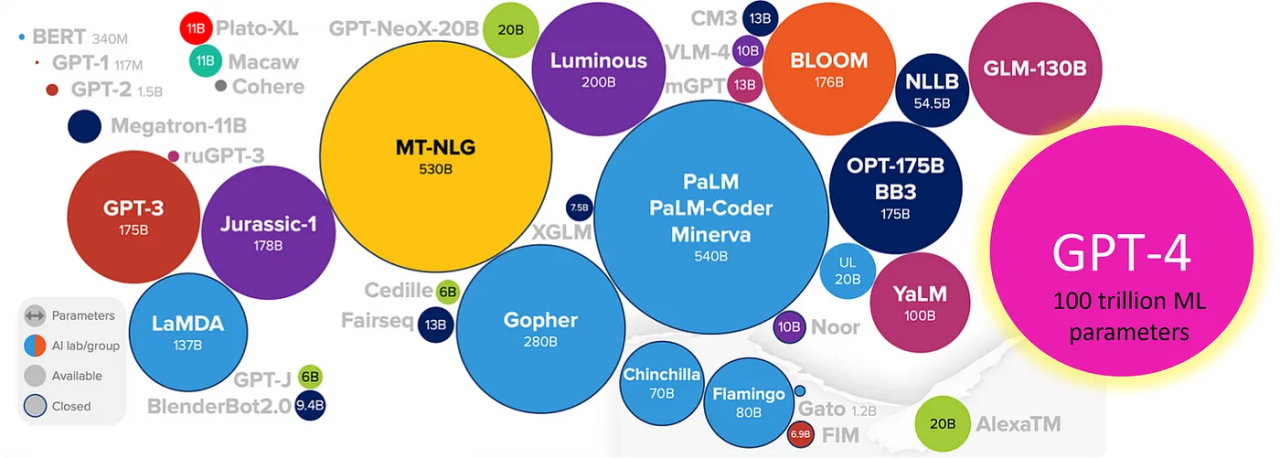
\includegraphics[width=0.9\textwidth]{./figuras/LLMs_sizes.png}
    \source{\cite{ChallengesAssociatedBuilding}}
    \label{fig:llm_sizes}
\end{figure}

\subsection{Modelos prentrenados y \textit{fine-tuning}} 
Bibliografía: \cite{chamandFinetuneYourClassifier2022}

Un \gls{llm} es entrenado desde cero con un gran corpus de textos de toda índole, normalmente tomados de internet: libros, blogs, artículos de periódicos, artículos científicos, \textit{wikis}, etc. El modelo, tras ese proceso, está \textit{prentrenado} \citep{hanPreTrainedModelsPresent2021} y puede ser utilizado, de forma genérica, para tareas de generación de texto, traducción automática, resumen de textos, etc. Sin embargo, es posible \textit{ajustar} (\textit{fine-tuning}) el modelo para que se adapte a un dominio específico, como la música, la programación, la medicina, etc., o a una tarea específica: dialogar en forma de \textit{chatbot}, ser amable, comportarse como un personaje concreto, etc. En este caso, el modelo se vuelve a entrenar con un corpus de textos específico del dominio, o con un conjunto de preguntas y respuestas con el estilo buscado, en el caso de ser un \textit{chatbot}. Todo ello permite que el modelo se adapte a ese dominio, mejore su capacidad predictiva o se comporte de la forma deseada \citep{tianFinetuningLanguageModels2023}. Este proceso de \textit{fine-tuning} es más rápido y requiere menos datos que el entrenamiento desde cero, por lo que es una opción muy interesante para adaptar los \gls{llm} a dominios específicos.

El \textit{fine-tuning} produce buenos resultados gracias a la capacidad de generalización de los \textit{llm} y de transformar el conocimiento adquirido (en el prentrenamiento) de un dominio a otro. Por ejemplo, un modelo entrenado con textos de biología puede ser \textit{ajustado} para que genere textos de medicina, o viceversa. El mecanismo por el que un aprendizaje se transforma en otro se denomina \textit{transfer learning} \citep{zhuangComprehensiveSurveyTransfer2020} y es una de las características más interesantes de los \gls{llm} (ver Figura \ref{fig:transfer_learning}).

\begin{figure}[H]
    \caption[Ejemplos intuitivos de \emph{Transfer learning} en \gls{llm}]{Ejemplos intuitivos de \emph{Transfer learning} en \gls{llm}. La capacidad de generalización de los \gls{llm} permite trasladar conocimientos y destrezas de un dominio a otro, especialmente si existe una relación o analogía entre ellos.}
    \centering
    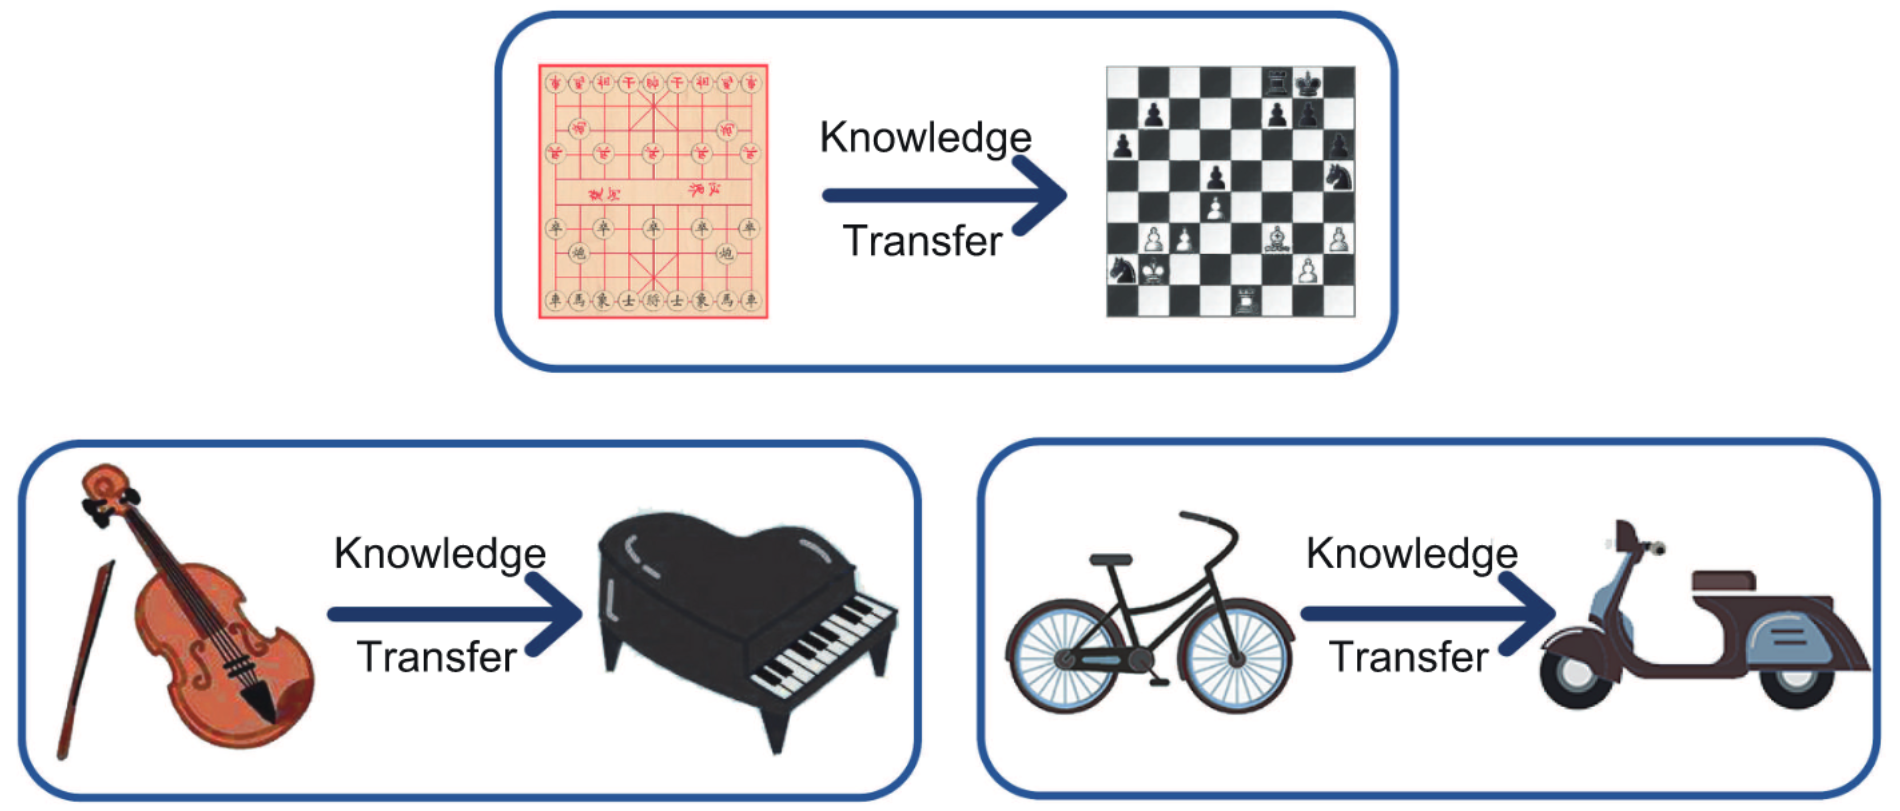
\includegraphics[width=0.6\textwidth]{./figuras/transfer_learning.png}
    \source{\cite{zhuangComprehensiveSurveyTransfer2020}}
    \label{fig:transfer_learning}
\end{figure}


\subsection{Hiperparámetros y parámetros del modelo}


Se denominan \textit{hiperparámetros} a los parámetros que se fijan de forma previa al entrenamiento del modelo, delimitando su estructura y capacidades computacionales \citep{QueEsAjuste}. Así, la arquitectura elegida, las dimensiones de cada una de sus partes, la tasa de aprendizaje, etc. Todo ello determinará las características del modelo entrenado, así como las necesidades de recursos computacionales necesarios tanto para la fase de entrenamiento como de inferencia.

Cuanto mayor sea el modelo, más parámetros variables tendrá en su entrenamiento, por lo que mayor costo computacional demandará. Actualmente, los \gls{llm} tienen un número de parámetros absolutamente prohibitivo dentro de la computación personal, del orden del billón \citep{radfordLanguageModelsAre2019}, por lo que su entrenamiento se realiza en \textit{clusters} de ordenadores de alto rendimiento, con cientos de GPUs. Sin embargo, una vez entrenados, son potencialmente utilizables en ordenadores personales para tareas de inferencia, como la generación de texto, traducción automática, etc., aunque lo más habitual es ofrecer sus servicios a demanda.

Además del número de parámetros, el tamaño de la ventana de contexto es otro hiperparámetro a considerar en un \gls{llm}. Este dato hace referencia a la cantidad de \textit{tokens} que un \gls{llm} puede recibir como input para realizar la inferencia del siguiente \textit{token}. 





Precisamente el número de parámetros y la ventana de contexto son los hiperparámetros más importantes y críticos en términos computacionales y de efectividad. Cuanto más grande sea el modelo, más parámetros tendrá y más capacidad de generar textos tendrá. Sin embargo, también será más lento en la inferencia. Por otro lado, cuanto mayor sea la ventana de contexto, más \textit{tokens} tendrá en cuenta el modelo para generar el siguiente \textit{token}, y más coherentes serán los textos generados. Sin embargo, también será más lento en la inferencia.


Consideraciones interesantes sobre parámetros y ventana de contexto en \cite{gonzaloAsomandonosVentanaContextual2023}

\subsection{Hiperparámetros controlables por el usuario}
\label{sec:hiperparametros_controlables}
Hablar de la temperatura, top\_p, top\_k, ventana de contexto, número de \textit{tokens}, etc. 

Se habla de la temperatura y su impacto en la generación de textos en \cite{holtzmanCuriousCaseNeural2020} y \cite{chamandFinetuneYourClassifier2022}

\cite{holtzmanCuriousCaseNeural2020} habla de la importancia de top\_p, en lo que denomina \textit{top\_k nucleus sampling}. Aunque es antiguo el paper, echar un ojo porque aclara bastante los conceptos.

Seguimos las explicaciones de \cite{rothmanTransformersNaturalLanguage2021}

Existen estudios centrados en la optimización de los hiperparámetros (los ya citados más arriba y \cite{wangCostEffectiveHyperparameterOptimization2023} y \cite{wangHyperparameterOptimizationAlgorithm2022})

